\section{Node Stack}
The node stack is implemented in the programming language D with some C libraries for crypto functions. It is structured, as shown in the figure below. 

\begin{table}[H]
{%
\newcommand{\mc}[3]{\multicolumn{#1}{#2}{#3}}
\begin{center}
\begin{tabular}{|c|c|}
\hline
\mc{2}{|c|}{HRPC (HiBON) Dataformat for communication}\\
\hline
\mc{2}{|c|}{NODE}\\
\hline
User API - TLS 1.2 & P2P Network\\
\hline
\mc{2}{|c|}{Scripting Engine}\\
\hline
\mc{2}{|c|}{Consensus mechanism : Hashgraph}\\
\hline
\mc{2}{|c|}{Storage : Distributed Database DART }\\
\hline
\mc{2}{|c|}{Storage state : Blockchain} \\
\hline
\end{tabular}
\end{center}
}%
\caption{Tagion Node stack}
\label{tab:node_stack}
\end{table}


A Tagion Node is divided into units as shown in \cref{fig:node_service} and each unit handles a service function in the following manner:

A smart-contract is sent to the Transaction-service-unit fetching the inputs from the DART unit and verifying their signatures. The DART-unit connects to other DARTs via the P2P-unit. The transaction-unit forwards the smart-contract including the inputs to the Coordinator-unit and this unit adds it to an event that is gossiped to the network via the P2P-unit.\\
When the Coordinator receives an event with a smart-contract, it is executed via the Scripting-Engine-unit, and the results of the outputs are verified.\\ 
When the Coordinator finds an epoch, this epoch is forwarded to the Transcript-service-unit that evaluates the correct order and requests the DART-unit to erase the inputs and add the newly generated outputs.

\begin{figure}[H]
 \centering
 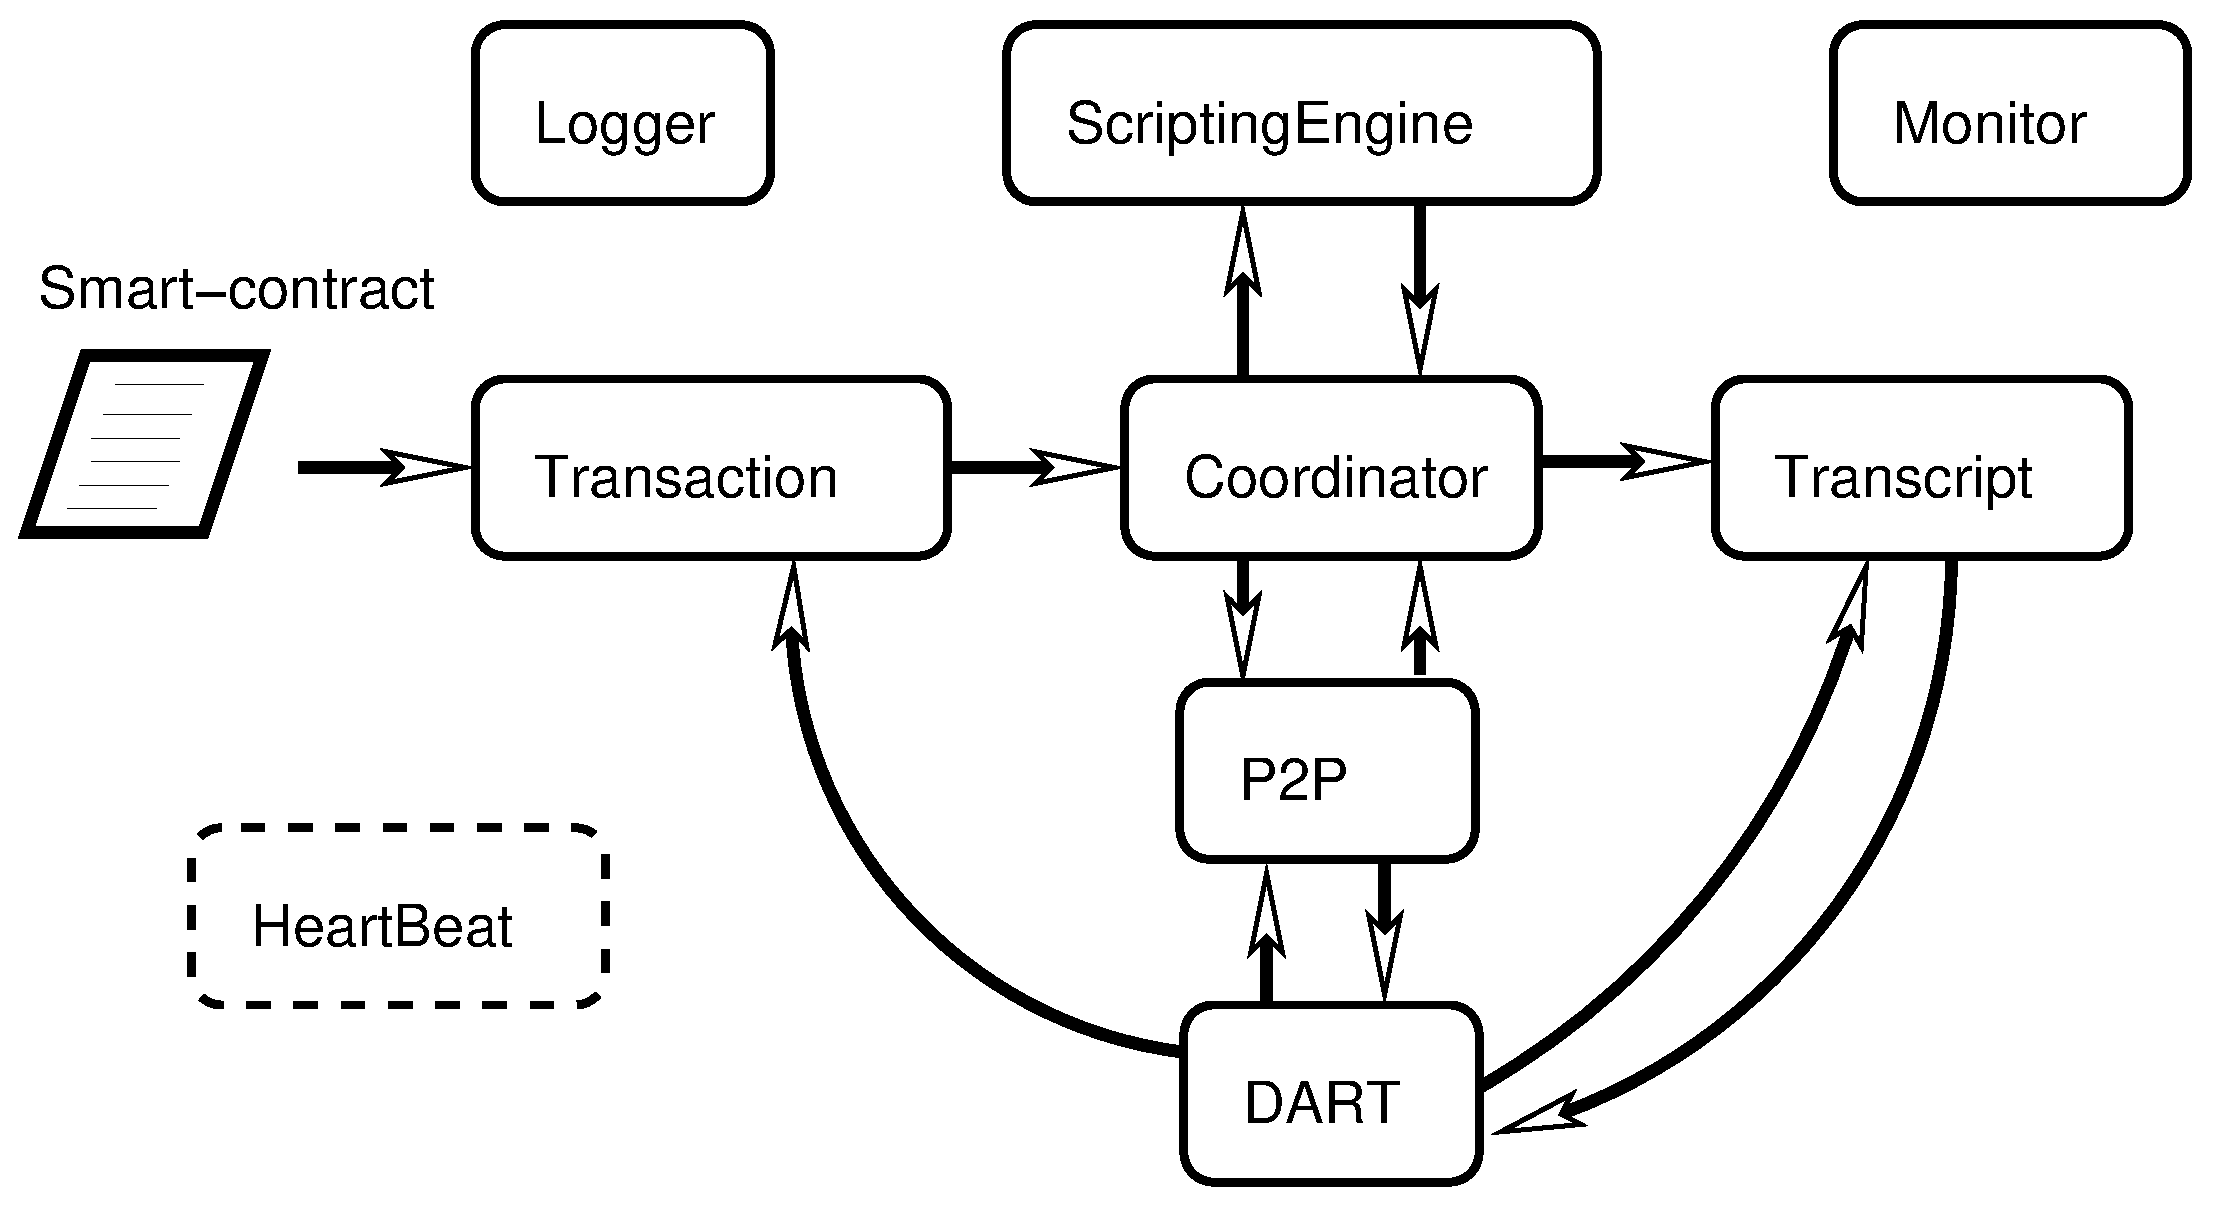
\includegraphics[width=0.8\textwidth]{fig/node_service.eps}
 % dart_bw.eps: 17766x12625 px, 300dpi, 150.42x106.89 cm, bb=0 0 4264 3030
 \caption{The Tagion Node service structure}
 \label{fig:node_service}
\end{figure}


Each of the services is running as independent tasks and communication between each-other via commutation channels. The different services modules perform the service as described in the list below.

\begin{itemize}
 \item[\bfit{Coordinator}] This service manages the hashgraph-consensus and controls other related service for the node. 
 The Coordinator generates and receives events and relays to the network. This service also generates the epoch and sends the information to the ScriptingEngine services.
 \item[\bfit{Transaction}] This service receives the incoming transaction script, validates, verifies and fetches the data from the DART and sends the information to the Coordinator.
 \item[\bfit{DART}] Services to the Distributed-database
 \item[\bfit{P2P}] This service handles the peer-to-peer communication protocol used to communicate between the nodes
 \item[\bfit{ScriptingEngine}] Handles the executions of the scripts
 \item[\bfit{Transcript}] Services the Epoch and orders the script execution
 \item[\bfit{Logger}] The service handles information logging for the different services
 \item[\bfit{Monitor}] The Monitor service is used to monitor the activities locally
 \item[\bfit{HeartBeat}] This service is only used in test-mode. This service enables the nodes to execute sequentially, simplifying network debugging.
 \end{itemize}
